\documentclass{article}

\usepackage[spanish]{babel}
\usepackage[numbers,sort&compress]{natbib}
\usepackage[T1]{fontenc}
\usepackage[ansinew]{inputenc}
\usepackage{graphicx}
\usepackage{url}
\usepackage{subcaption}
\usepackage{caption}
\usepackage{listings}
\usepackage{amsmath}
\usepackage{float}
\usepackage[numbers,sort&compress]{natbib}

\begin{document}
\title{\textbf{Interacciones entre part\'iculas}}
\author{Anahi Elizabeth Llano}

\maketitle

\section{Objetivo}\label{obj}

El objetivo de la practica \cite{elisa} consiste en simular la interacci\'on de las part\'iculas teniendo en cuenta su carga, masa y las fuerzas de atracci\'on y repulsi\'on, as\'i como la gravedad para realizar un an\'alisis en la distribuci\'on de la velocidad de tales part\'iculas.


\section{Metodolog\'{i}a}\label{met}

Se realizo una modificaci\'on del ultimo c\'odigo mostrado en clase \cite{elisa}, utilizando una versi\'on de Python 3.7, de tal manera de poder llevar a cabo la simulaci\'on, en donde para la rutina, se utilizaron $50$ part\'iculas cada una de ellas con carga aleatoria que va desde entre $-1 y +1$ agregando de igual manera una masa aleatoria, en un total de $100$ pasos. Se sabe que las cargas que posean un mismo signo  generaran fuerzas de repulsi\'on y las cargas de signos contrarios producen fuerzas de atracci\'on, donde de manera adicional se estar\'a presentando la gravedad ejerciendo una fuerza la cual ser\'a mayor conforme vaya en aumento la masa.
Para el an\'alisis de resultados se realizaron histogramas \citep{daliadisc}, as\'i como una matriz de dispersi\'on \citep{elitedisc} para observar el comportamiento de las part\'iculas de acuerdo con las distintas variables tomadas en cuenta.

\section{Resultados y Discusi\'{o}n}\label{res}
 
En la figura \ref{f1} se observa el paso 1 de las part\'iculas a partir de esta imagen se encuentra en el repositorio  \citep{ana} el gift resultante de las $100$ interacciones. As\'i mismo en la figura  \ref{f1} se observa la matriz de dispersi\'on en donde se observa que para todas las variables las part\'iculas se encuentran dispersas donde las variables $x$ es la posici\'on en $x$, $y$ es la posici\'on en $y$, $c$ es la carga y $m$ es la masa de las part\'iculas.

\begin{figure}[H]
       \centering
       \begin{subfigure}[b]{0.70\linewidth}
           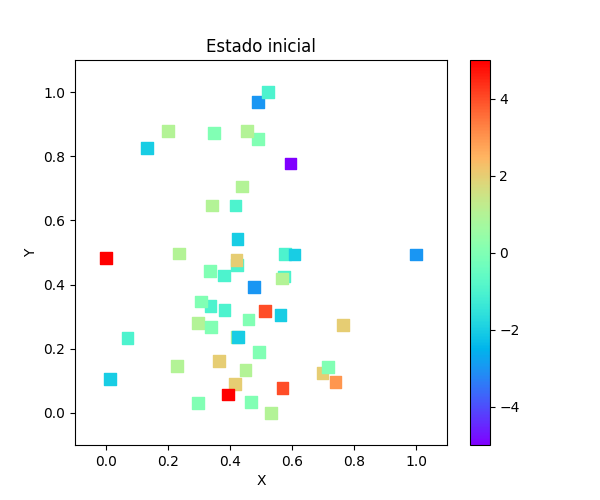
\includegraphics[width=\linewidth]{p9p_t0.png}
           \caption{paso 1}
           \label{f1.a}
        \end{subfigure}
\begin{subfigure}[b]{0.70\linewidth}
           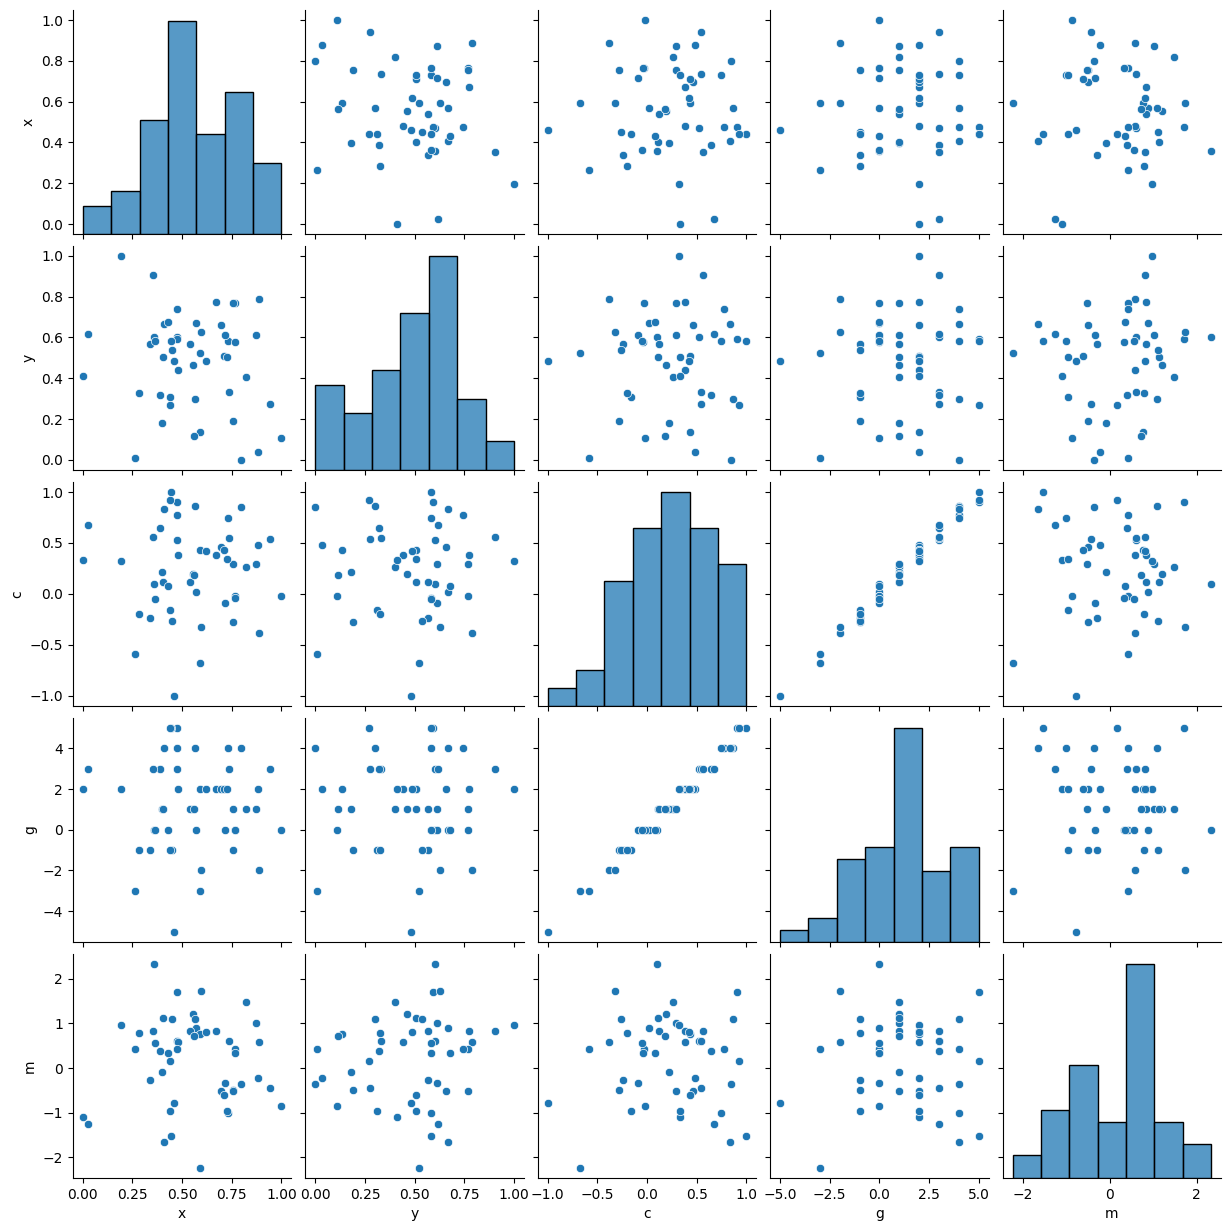
\includegraphics[width=\linewidth]{tiempsop_t001.png}
           \caption{paso 1}
           \label{f1.b}
        \end{subfigure}
\caption{Paso 1}
        \label{f1}
\end{figure}

Mediante histogramas se observan las diferentes variables en donde vemos en la figura \ref{f2} que  las cargas permanecen constantes.

\begin{figure}[H]
       \centering
       \begin{subfigure}[b]{0.60\linewidth}
           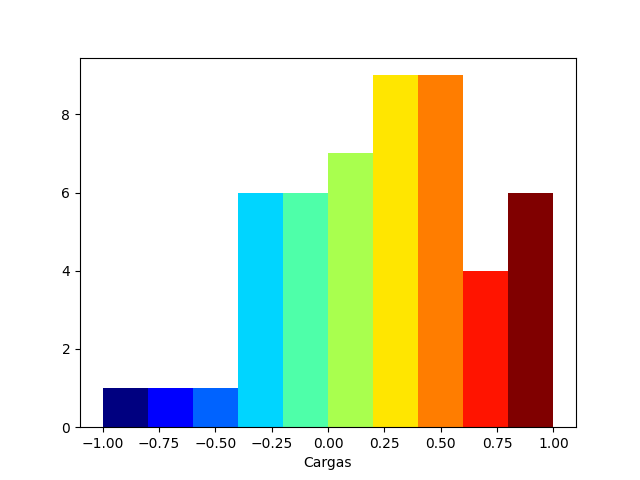
\includegraphics[width=\linewidth]{p9carga_t001.png}
           \caption{paso 1}
           \label{f1.a}
        \end{subfigure}
 \begin{subfigure}[b]{0.60\linewidth}
           \includegraphics[width=\linewidth]{p9carga_t100.png}
           \caption{paso 100}
           \label{f1.b}
        \end{subfigure}
\caption{Carga de las part\'iculas}
        \label{f2}
\end{figure}

As\'i mismo en la figura \ref{f3} las masas asignadas  permanecen de igual manera constantes conforme aumenta el n\'umero de interacci\'on.

\begin{figure}[H]
       \centering
       \begin{subfigure}[b]{0.60\linewidth}
           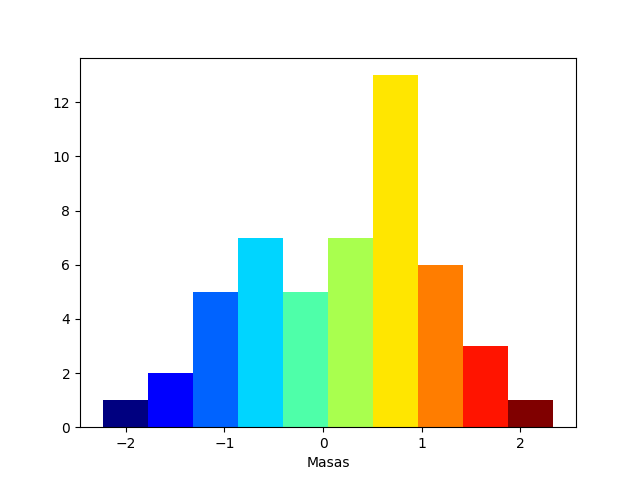
\includegraphics[width=\linewidth]{p9masa_t001.png}
           \caption{paso 1}
           \label{f1.a}
        \end{subfigure}
 \begin{subfigure}[b]{0.60\linewidth}
           \includegraphics[width=\linewidth]{p9masa_t100.png}
           \caption{paso 100}
           \label{f1.b}
        \end{subfigure}
\caption{Masa de las part\'iculas}
        \label{f3}
\end{figure}


Con apoyo de la matriz de dispersi\'on observamos todas las variables mencionadas con respecto a los diferentes tiempos, en la figura  \ref{f4} lo observamos para tiempos de $25$, $50$, $75$ y $100$.

\begin{figure}[H]
       \centering
        \begin{subfigure}[b]{0.45\linewidth}
            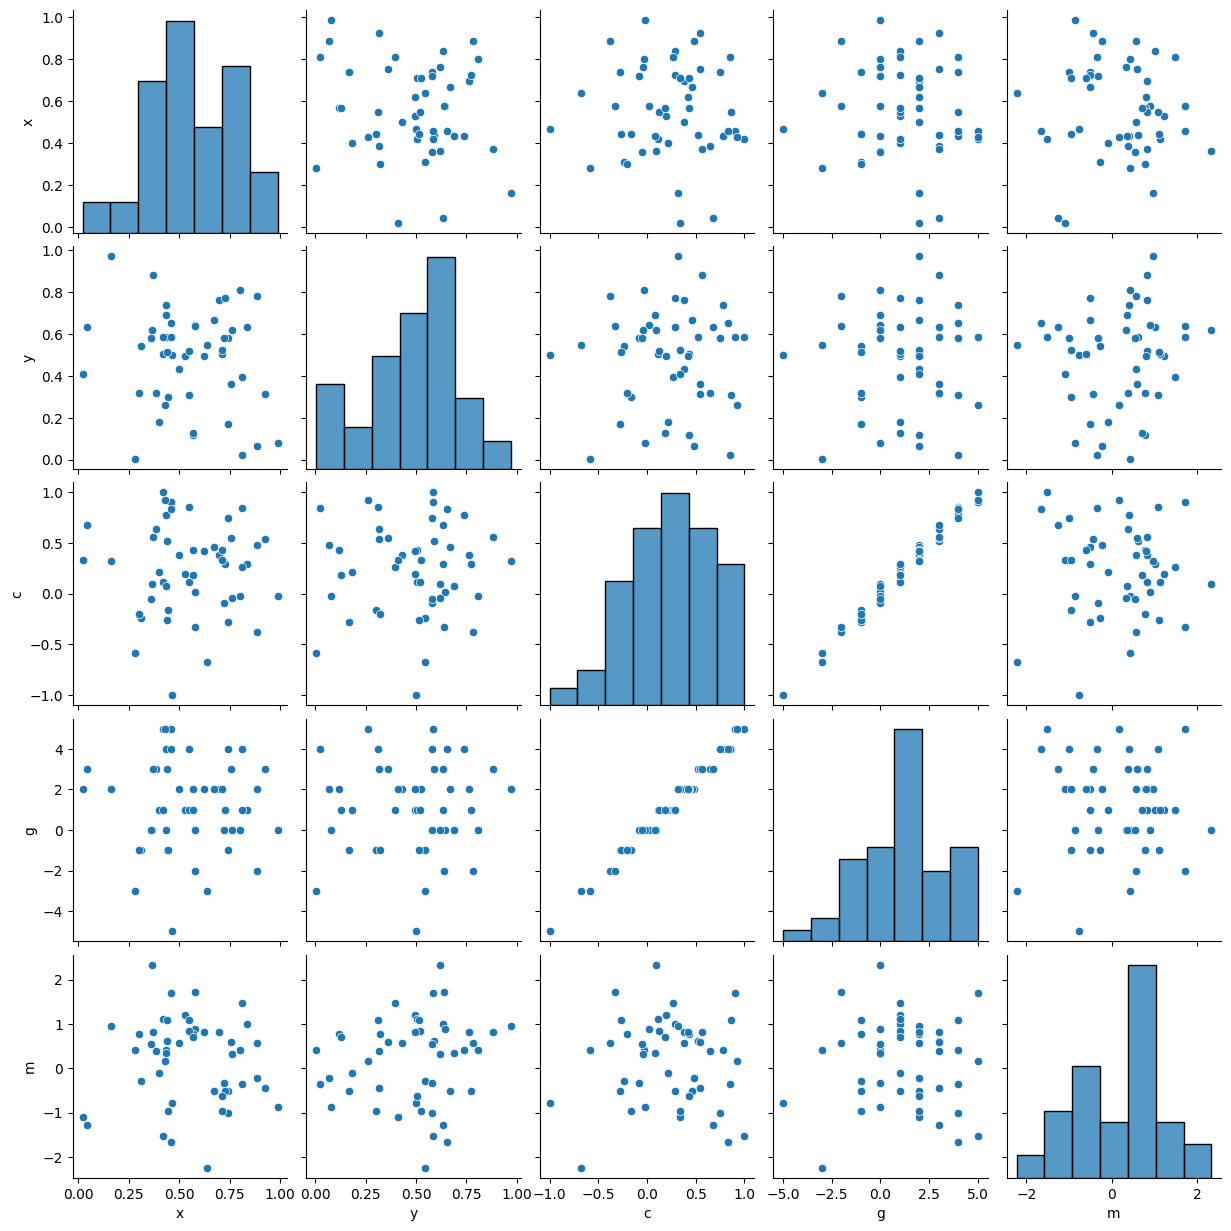
\includegraphics[width=\linewidth]{tiempsop_t025.png}
            \caption{paso 25}	
            \label{f2.a}
        \end{subfigure}
\begin{subfigure}[b]{0.45\linewidth}
            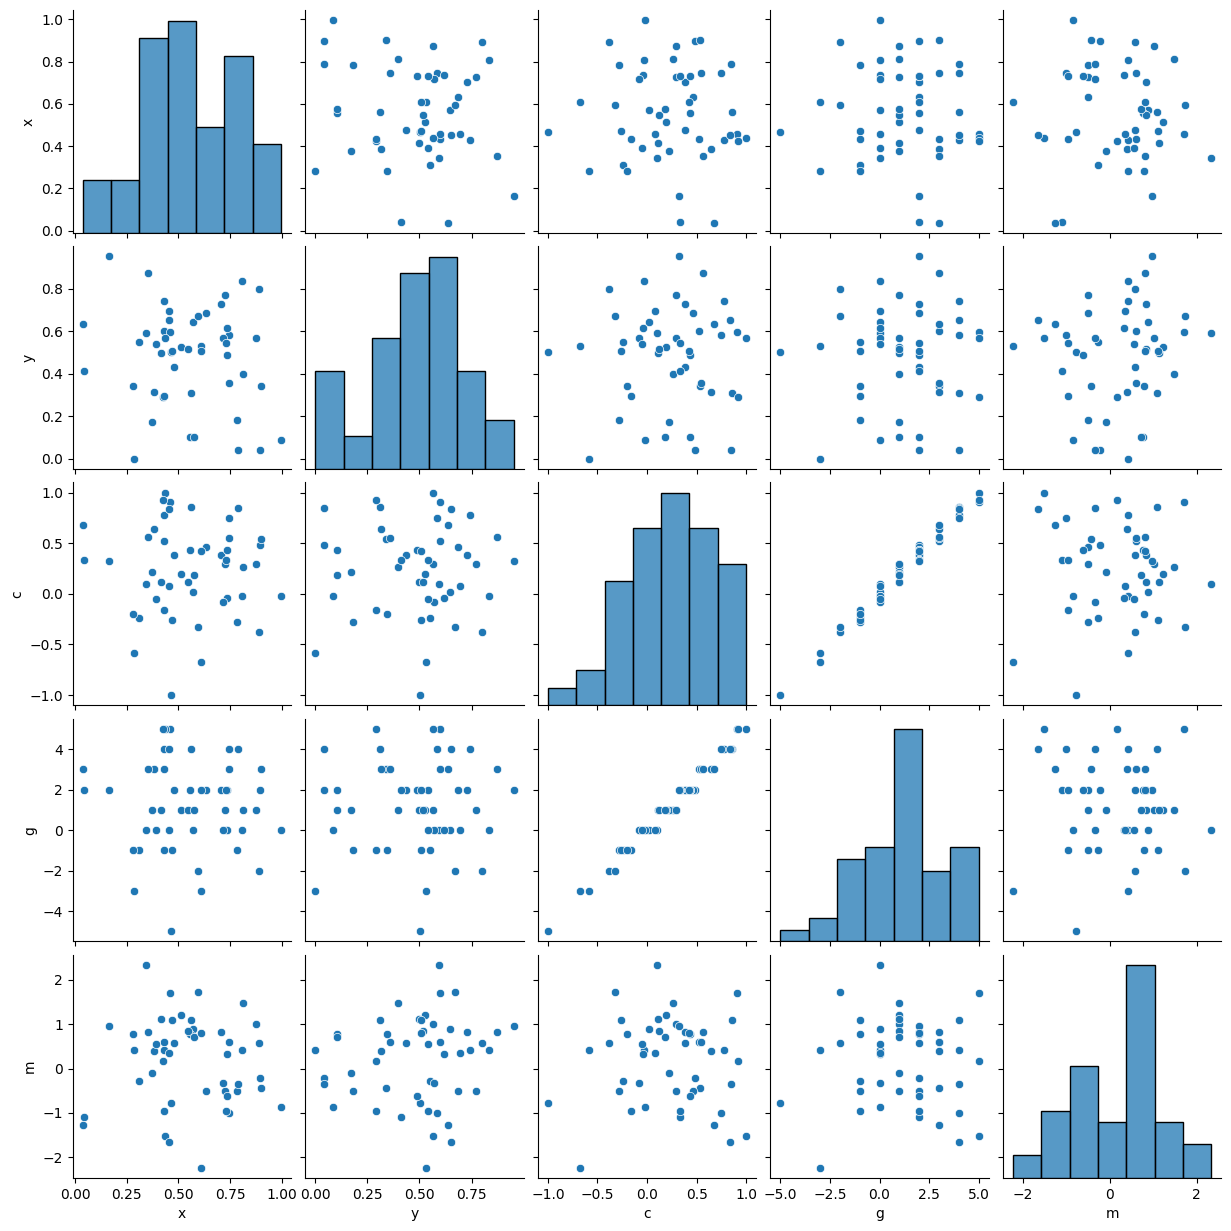
\includegraphics[width=\linewidth]{tiempsop_t050.png}
            \caption{paso 50}
            \label{f2.b}
        \end{subfigure}
\begin{subfigure}[b]{0.45\linewidth}
            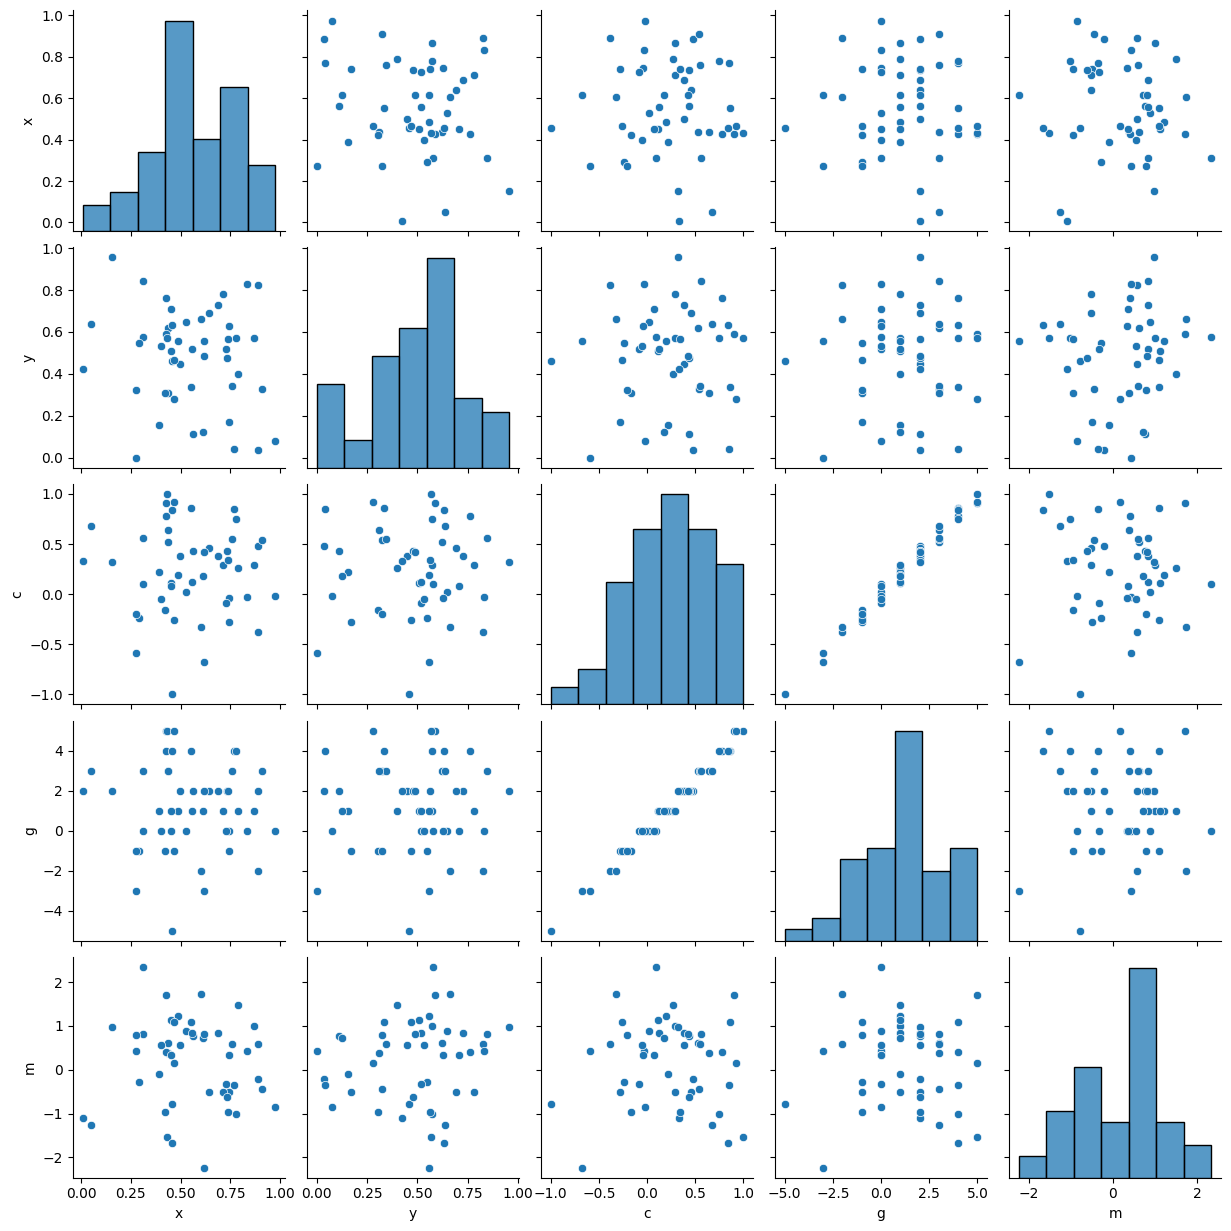
\includegraphics[width=\linewidth]{tiempsop_t075.png}
            \caption{paso 75}
            \label{f2.b}
        \end{subfigure}
\begin{subfigure}[b]{0.45\linewidth}
            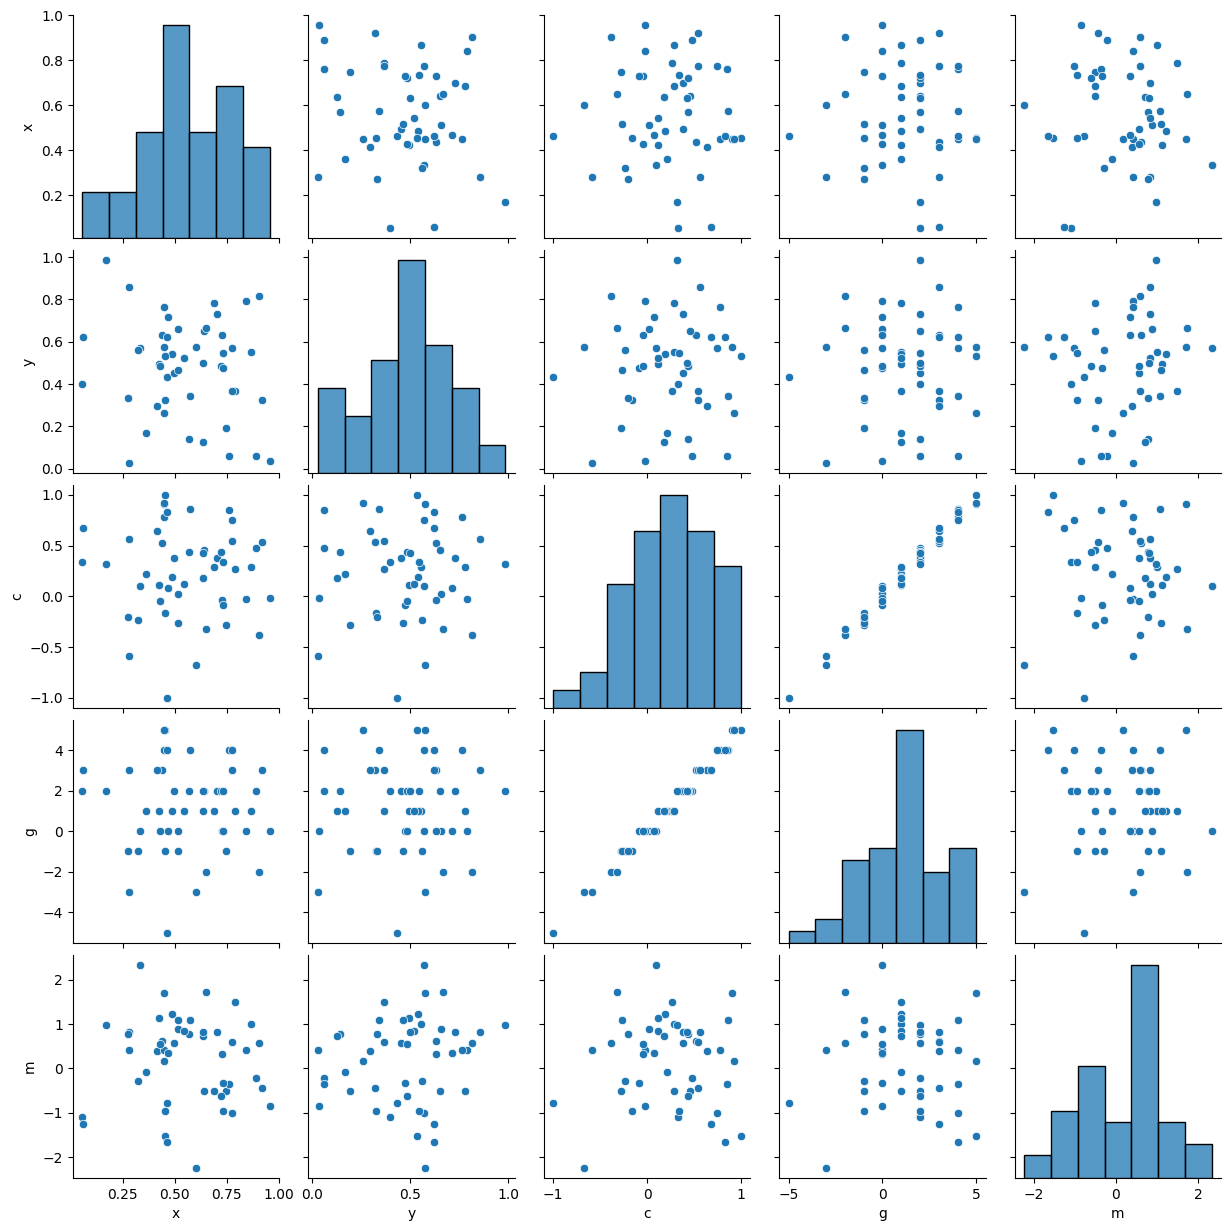
\includegraphics[width=\linewidth]{tiempsop_t100.png}
            \caption{paso 100}
            \label{f2.b}
        \end{subfigure}
\caption{Matriz de dispersi\'on en diferentes tiempos}
        \label{f4}
\end{figure}

Finalmente, mediante el uso de histogramas se obtuvo un promedio de las velocidades obtenidas durante la simulaci\'on el cual se observa en la figura  \ref{f5}

\begin{figure}[H]
       \centering
           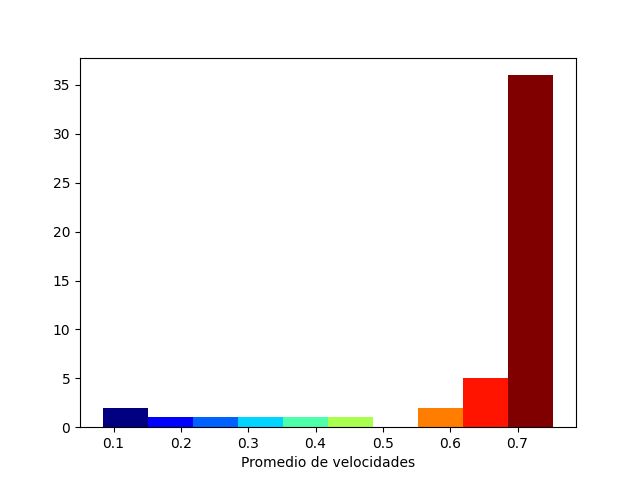
\includegraphics[width=0.90\linewidth]{promediovelocidades.png}
           \caption{Promedio de las velocidades}
           \label{f5}
\end{figure}

\begin{figure}
       \centering
        \begin{subfigure}[b]{0.45\linewidth}
            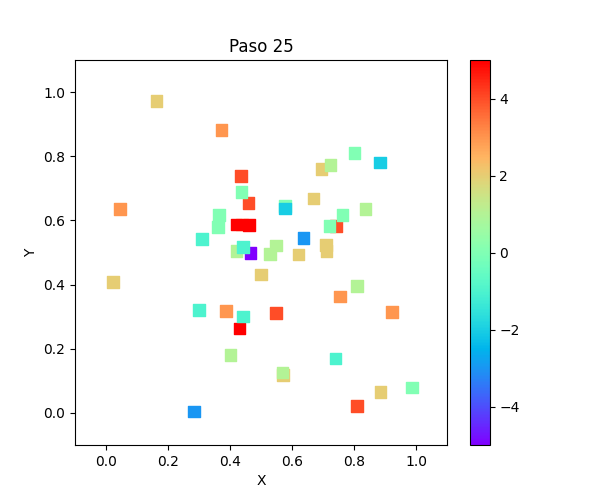
\includegraphics[width=\linewidth]{p9p_t025.png}
            \caption{paso 25}	
            \label{f2.a}
        \end{subfigure}
\begin{subfigure}[b]{0.45\linewidth}
            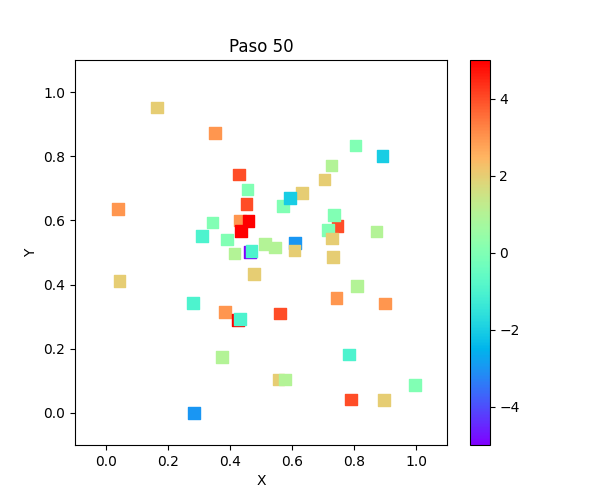
\includegraphics[width=\linewidth]{p9p_t050.png}
            \caption{paso 50}
            \label{f2.b}
        \end{subfigure}
\begin{subfigure}[b]{0.45\linewidth}
            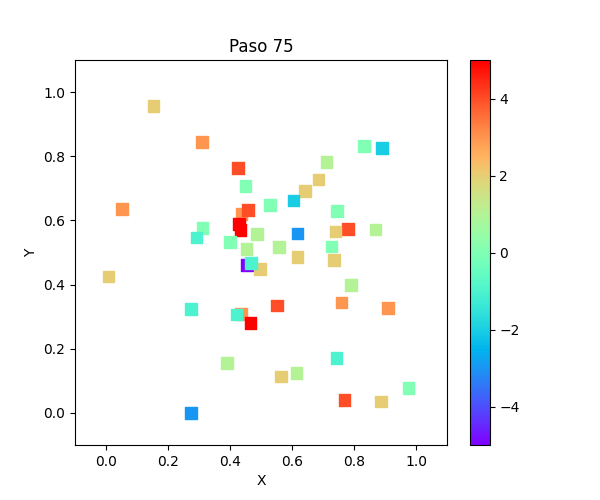
\includegraphics[width=\linewidth]{p9p_t075.png}
            \caption{paso 75}
            \label{f2.b}
        \end{subfigure}
\begin{subfigure}[b]{0.45\linewidth}
            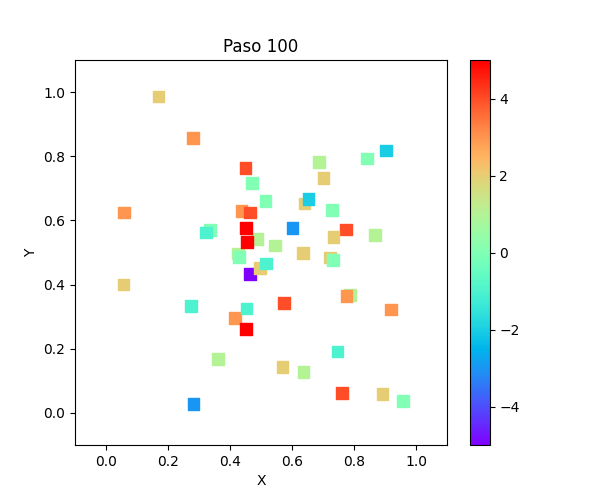
\includegraphics[width=\linewidth]{p9p_t100.png}
            \caption{paso 100}
            \label{f2.b}
        \end{subfigure}
\caption{Interaccion entre part\'iculas}
        \label{f6}
\end{figure}

\section{Conclusi\'{o}n}\label{con}

En la simulaci\'on realizada se concluye que tenemos diferentes par\'ametros que afectan ya sea de manera positiva o negativa en la interacci\'on entre part\'iculas, algo que se pudo observar es que la masa y la carga de estas permanec\'ia constante conforme aumentaba el tiempo, mientras la masa de las part\'iculas sea menor la velocidad de estas tambi\'en ser\'a menor, por lo cual se puede suponer que existe una relaci\'on entre ambos.


  \bibliography{P9}
  \bibliographystyle{plainnat}
\end{document}